\chapter{深層学習における二重降下現象}
\section{はじめに}
本研究では,深層学習における二重降下現象を観察するためにNakkiranら\cite{nakkiran2021deep}の条件を使用している.本章では,学習時における具体的な実験設定を述べるとともに,その条件を使用したModel-wise Double Descent, Epoch-wise Double Descentの追試結果を示す.

\section{Nakkiran's setting}
\label{sec:Nakkiran's setting}
% PyTorchで利用可能なImageNetで事前学習された重みを持つResNet18を使用し,CIFAR-10~\cite{Krizhevsky2009_cifar}で学習させる.学習データにはラベルノイズとデータ拡張を加える.ラベルノイズは,学習データの正しいラベルを$p$の確率でランダムに別のラベルに変更する.データ補強では,画像の上下左右に4ピクセルのマージンを加え,32x32のサイズにトリミングし,画像をランダムに水平反転させる.バッチサイズを128に設定し,損失関数としてCrossEntropyLossを用いる.最適化にはAdam~\cite{Adam}を用い,学習率は0.0001とする.
ResNet18を使用し,CIFAR-10~\cite{Krizhevsky2009_cifar}を学習させる.学習データにはラベルノイズとデータ拡張を加える.ラベルノイズは,学習データの正しいラベルを$p$の確率でランダムに別のラベルに変更する.データ補強では,画像の上下左右に4ピクセルのマージンを加え,32x32のサイズにトリミングし,画像をランダムに水平反転させる.バッチサイズを128に設定し,損失関数としてCrossEntropyLossを用いる.最適化にはAdam~\cite{Adam}を用い,学習率は0.0001とする.

\subsection{Model-wise Double Descent}
一般的なResNet18の各ブロックの出力チャネル数が[64, 128, 256, 512]であるのに対し,[1$\times k$, 2$\times k$, 3$\times k$, 4$\times k$]と横幅を可変にすることでパラメータ数を制御し二重降下を観察している.以降横幅可変なResNet18をResNet18kと呼称する.ラベルノイズは$p=0.15$として,$k=1\sim64$に設定したResNet18kをそれぞれ4,000 epoch学習させ,最終的なテスト誤り率をグラフに図示する.実際の結果を\cref{fig:DD}に示す.$k=5$,$k=10$の付近でテスト誤り率が下降から上昇,上層から下降と切り替わり,二重降下の曲線が観察できる.

\begin{figure}[ht]
    \centering
    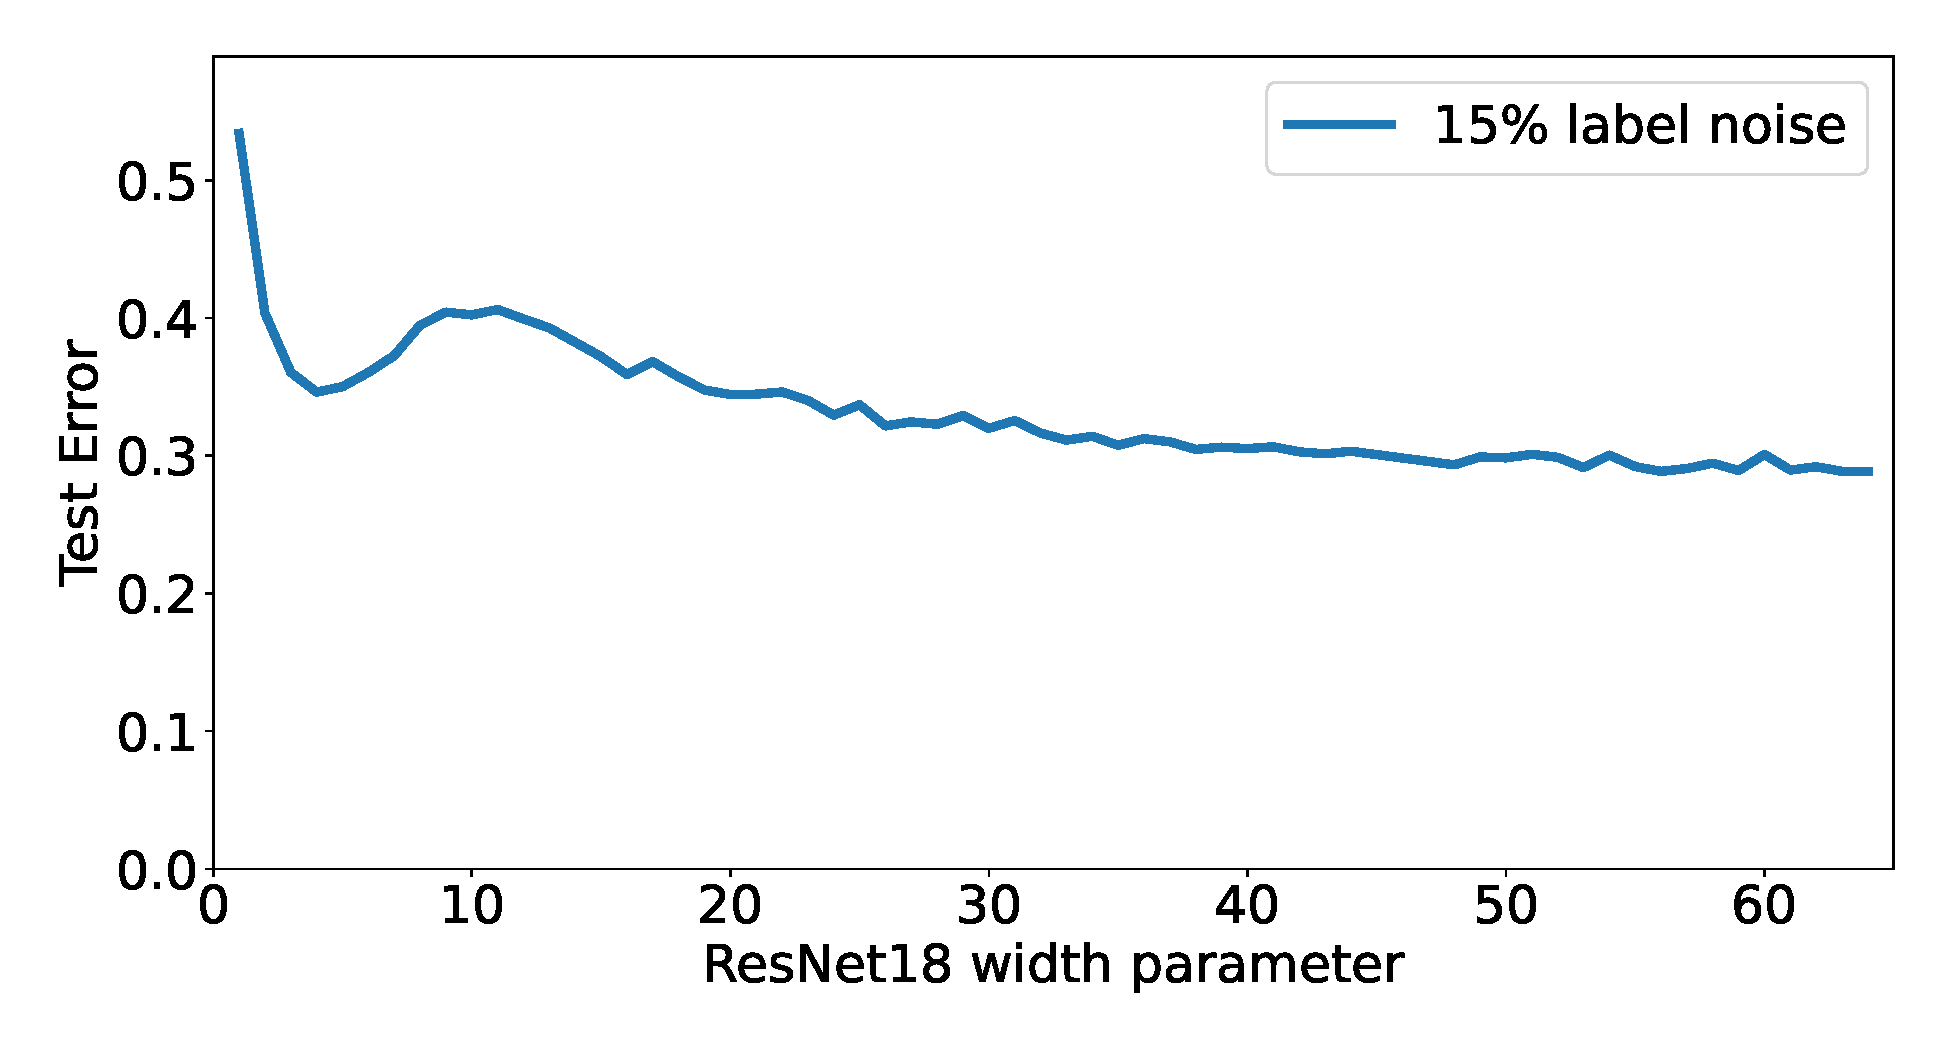
\includegraphics[width=1\columnwidth]{fig/DoubleDescent.pdf}
    \caption{Model-wise Double Descent by Nakkiran's setting}
    \label{fig:DD}
\end{figure}

\newpage

\subsection{Epoch-wise Double Descent}
先述した,ResNet18kを$k=128$で使用し,同様に4,000epoch学習させ,学習過程のテスト誤り率の推移を観察する.実際の結果を\cref{fig:EDD}に示す.20から30epoch目,60から70epoch目付近でテスト誤り率が下降から上昇,上層から下降と切り替わり,二重降下の曲線が観察できる.

以降の実験では,一般的なResNet18($k=64$に設定したResNet18kとほぼ同等)を先述した条件で学習,学習過程における二重降下を観察している.

\begin{figure}[ht]
    \centering
    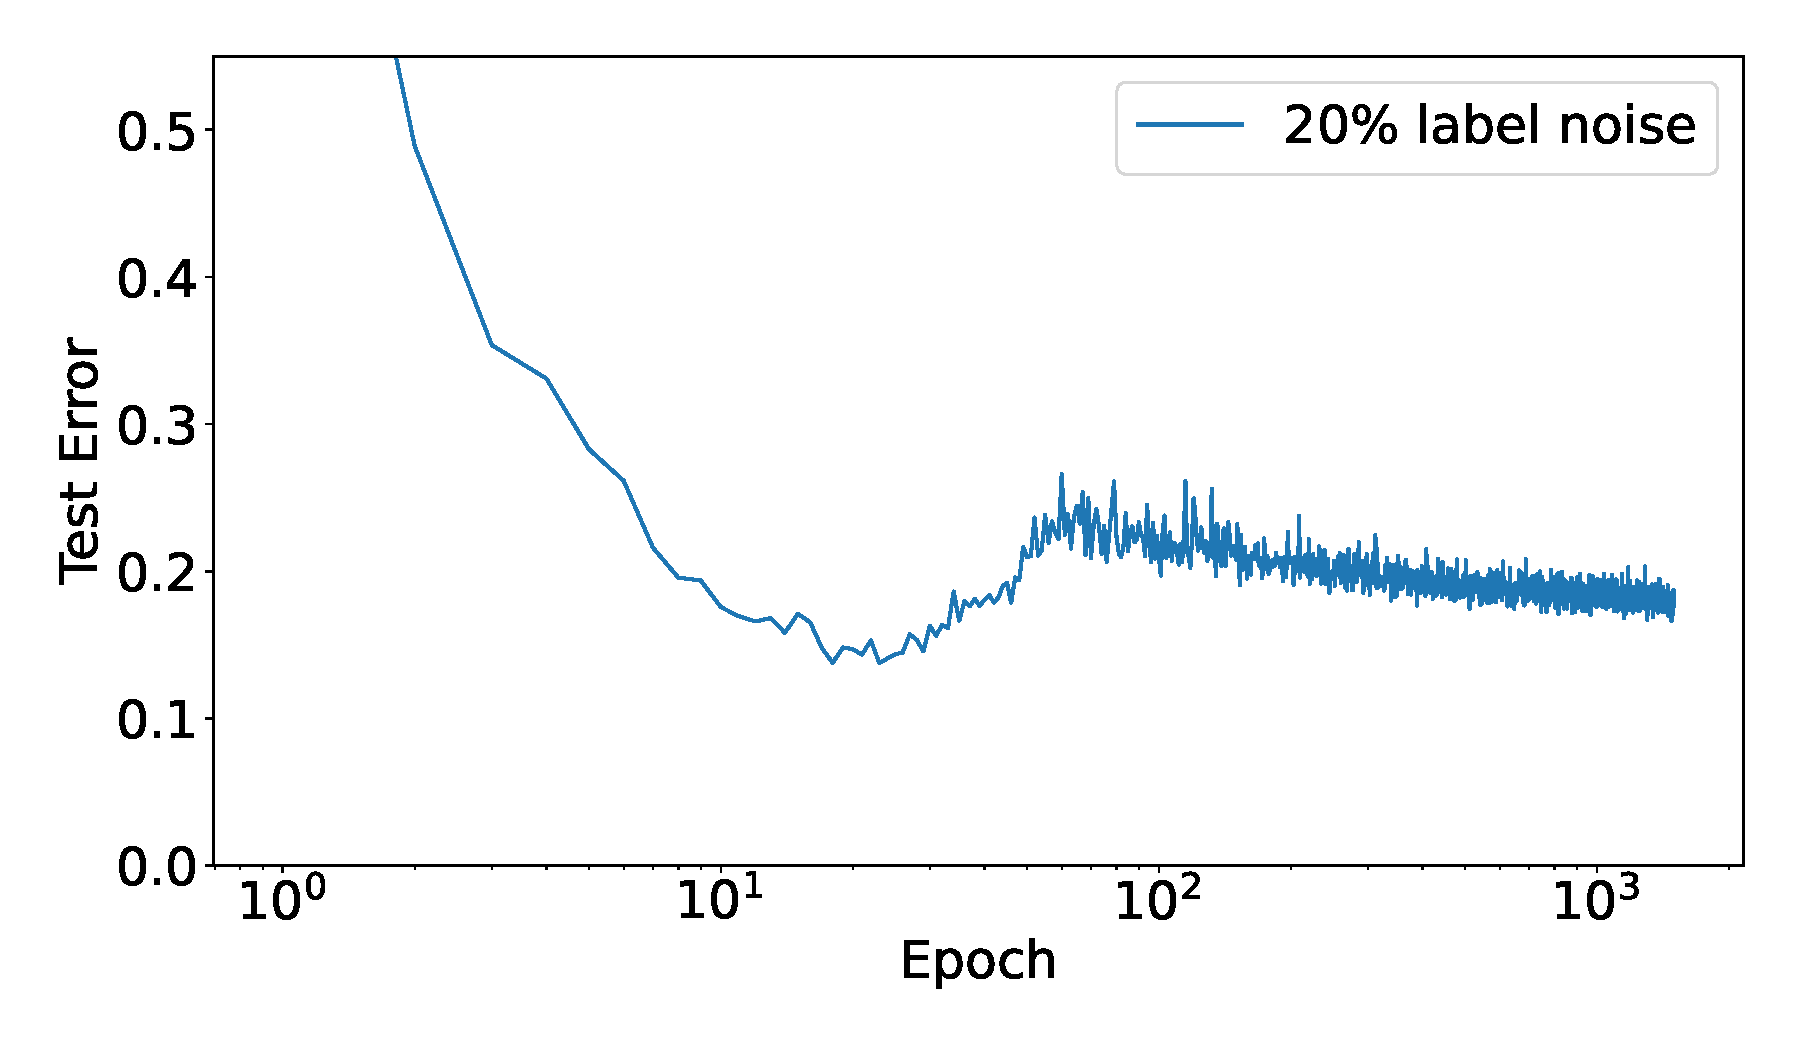
\includegraphics[width=1\columnwidth]{fig/Epoch-wise_DoubleDescent.pdf}
    \caption{Epoch-wise Double Descent by Nakkiran's setting}
    \label{fig:EDD}
\end{figure}

\newpage